\chapter{Concepts}

\section{Ensembles, langages, relations et fonctions}

\subsection{Ensembles}

Un \blue{ensemble} est une collection d'objets, sans répétition, appelés les éléments de l'ensemble.\\
Exemples : ensemble vide = $\emptyset$, ensemble fini = $\{1, 2, 3\}$, ensemble infini = $\{1, 2, 3, ...\}$, complément de $A = \bar{A}$.

\subsection{Langages}

Un \blue{langage} est un ensemble de mots constitués de symboles d'un \blue{alphabet} donné.\\
Exemple : palindromes sur $\{a, b\}$ : $\epsilon, a, b, aa, aaa, baab, babab, ...$

Un \blue{alphabet $\Sigma$} est un ensemble de symboles.\\
Exemples : $\Sigma = \{0, 1\}, \Sigma = \{a, b, c\}$

Une \blue{chaîne de caractères}, ou mot, est une séquence finie de symboles juxtaposés.\\
Exemples : $010110, abccbcabcb, \epsilon$ (= chaîne de caratères vide)\\
L'ensemble de tous les mots de l'\blue{alphabet $\Sigma$} s'écrit $\Sigma^*$\\
Exemples : $\Sigma = \{\} \rightarrow \Sigma^* = \{\epsilon\}, \Sigma = \{a\} \rightarrow \Sigma^* = \{\epsilon, a, aa, aaa, aaaa, ...\}$

\subsection{Relations et fonctions}

Une \blue{relation} $R$ sur $A, B$ est un sous ensemble de $A$x$B$. En pratique, on dit que c'est une \blue{fonction}.

Une \blue{fonction $f$} (de A dans B) est une relation t.q. pour $a \in A$, il existe au plus un $b \in B$ t.q. $<a, b> \in f$.

\subsubsection{Propriétés des fonctions}

Soit $f : A \rightarrow B$ :
\begin{itemize}
\item \blue{Domaine} de $f$ : dom($f$) $= \{a \in A \ | \ f(a) \neq \bot\}$
\item \blue{Image} de $f$ = im($f$) $= \{b \in B \ | \ \exists a \in A : b = f(a)\}$
\item $f$ est fonction \blue{totale} ssi dom($f$) $= A \ (\nexists a \in A : f(a) = \bot)$ 
\item $f$ est fonction \blue{partielle} ssi dom($f$) $\subseteq A$ ($f$ totale est partielle mais $f$ partielle n'est pas forcément totale)
\item $f$ est \blue{surjective} ssi im($f$) $= B$ (tout $y$ a au moins un $x$)
\item $f$ est \blue{injective} ssi $\forall a, a' \in A : a \neq a' \rightarrow f(a) \neq f(a')$ (tout x a un y différent)
\item $f$ est \blue{bijective} ssi $f$ est totale, injective et surjective (tout y a un et un seul x)
\end{itemize}

\section{Ensembles énumérables}

Un ensemble est \blue{énumérable} s'il est soit fini ou s'il a le même \blue{cardinal}\footnote{Deux Ensembles $A$ et $B$ ont le même cardinal s'il existe une bijection entre $A$ et $B$.} que $\mathbb{N}$\footnote{Pour rappel, l'ensemble $\mathbb{N}$ est l'ensemble des entiers positifs $\mathbb{N} = \{0, 1, 2, 3, \ldots\}$.} (si on peut le mettre en bijection avec $\mathbb{N}$). En informatique, un programme est une chaîne finie de caractères $\rightarrow$ énumérable.

\subsubsection{Propriétés}

\begin{itemize}
\item Tout sous-ensemble d'un ensemble énumérable est énumérable
\item L'union et l'intersection de deux ensembles énumérables est énumérable
\item L'union d'une infinité énumérable d'ensemble énumérables est énumérable
\end{itemize}

\subsection{Diagonalisation de Cantor}

Soit $E = \{x \in \mathbb{R} \ | \ 0 < x \leq 1\}$. \blue{$E$ est non énumérable}\footnote{Il n'existe pas de bijection entre $E$ et $\mathbb{N}$ c.à.d. qu'il y a beaucoup plus de réels entre 0 et 1 qu'il n'y a d'entiers positifs.}

\blue{Preuve} :
\begin{enumerate}
\item Supposons $E$ énumérable. Il existe donc une énumération des éléments de $E : x_0, ..., x_k, ...$
\begin{figure}[H]
    	\centering
    	\begin{tabular}{c|cccccc}
	 & 1 digit & 2 digit & 3 digit & $\cdots$ & $k+1$ digit & $\cdots$ \\ 
	\hline 
	$x_0$ & $x_{00}$ & $x_{01}$ & $x_{02}$ & $\cdots$ & $x_{0k}$ & $\cdots$ \\ 
	$x_1$ & $x_{10}$ & $x_{11}$ & $x_{12}$ & $\cdots$ & $x_{1k}$ & $\cdots$ \\ 
	$x_2$ & $x_{20}$ & $x_{21}$ & $x_{22}$ & $\cdots$ & $x_{2k}$ & $\cdots$ \\ 
	$\vdots$ & $\vdots$ & $\vdots$ & $\vdots$ & $\ddots$ & $\vdots$ & $\cdots$ \\ 
	$x_k$ & $x_{k0}$ & $x_{k1}$ & $x_{k2}$ & $\cdots$ & $x_{kk}$ & $\cdots$ \\ 
	$\vdots$ & $\vdots$ & $\vdots$ & $\vdots$ & $\vdots$ & $\vdots$ & $\ddots$ \\ 
	\end{tabular}
	\caption{\red{Construire une table} t.q. le nombre $x_k = 0,x_{k0} x_{k1} x_{k2} \ldots x_{kk} \ldots$}
\end{figure}
\item \red{Prendre la diagonale} ($d = 0,x_{00} x_{11} x_{22} \ldots x_{kk} \ldots$)
\item \red{Modifier la diagonale} t.q.
\begin{equation*}
	x'_{ii}=
	\begin{cases}
      	5 & \text{si}\ x_{ii} \neq 5 \\
      	6 & \text{sinon}
    \end{cases}
\end{equation*}
Ce qui donne $d' =  0,x_{00}' x_{11}' x_{22}' \ldots x_{kk}' \ldots \ (d' \in E)$
\item \red{Contradiction} : Comme $E$ est énumérable, et que $d' \in E$, alors $d'$ doit être dans l'énumération. Or, si $d' = x_p$, on a :
\begin{align*}
	d' &= 0,x_{p0} x_{p1} x_{p2} \ldots x_{pp} \ldots\\
	   &= 0,x'_{p0} x'_{p1} x'_{p2} \ldots x'_{pp} \ldots
\end{align*}
\item \red{Conclusion} : $E$ n'est pas énumérable
\end{enumerate}

\bigskip

Avec ceci, on remarque qu'il existe des ensembles avec un cardinal plus grand que $\mathbb{N}$. Quelques un des ces ensembles sont : $\mathcal{P}(A)$, fonctions de $\mathbb{N} \rightarrow \mathbb{N}$, chaînes infinies sur un alphabet fini, etc. Le fait que les fonctions de $\mathbb{N} \rightarrow \mathbb{N}$ soient non énumérables (cfr. section \ref{sec:ensembleF}) nous dit que l'ensemble des problèmes a donc un plus grand cardinal que l'ensemble des programmes (ayant le même cardinal que $\mathbb{N}$).

\chapter{Résultats fondamentaux}

\section{Programmes et fonctions}

\subsection{Algorithme}

Un \blue{algorithme} est une procédure qui peut être appliquée à n'importe quelle donnée (appartenant à une classe de données symboliques) et qui a pour effet de produire un résultat (appartenant à une classe de données symboliques). C'est un ensemble fini d'instructions (programme) \blue{calculant} une fonction (algorithme $\neq$ fonction)

\subsection{Univers des programmes}

On se base sur un langage de programmation. Ex : les programmes Python (si une fonction est calculable, elle doit être calculable par une programme Python).

\subsection{Univers des fonctions}

On se limite aux fonctions de $\mathbb{N} \rightarrow \mathbb{N}$, et plus généralement de $\mathbb{N}^n \rightarrow \mathbb{N}$.

\section{Fonction calculable}

Une fonction $f : \mathbb{N} \rightarrow \mathbb{N}$ est calculable ssi il existe un programme Python qui, recevant comme données n'importe quel nombre naturel $x$, fourni comme résultat $f(x)$ s'il est défini, sinon $\bot$ (s'il ne se termine pas ou erreur).

\subsubsection{Remarques}

\begin{itemize}
\item Existence $\neq$ savoir l'écrire
\item Si non calculable $\rightarrow$ aucun programme ne peut la calculer
\item Généralisable pour $\mathbb{N}^n \rightarrow \mathbb{N}$
\end{itemize}

\subsection{Ensemble récursif}

On dit que l'ensemble $A$ est récursif ssi il existe un programme qui prend en input $x$ et qui renvoi (c.à.d un ensemble récursif est un ensemble pour lequel on est capable de dire si un élément y appartient) :

$\begin{cases}
	1 & \text{si}\ x \in A\\
	0 & \text{si}\ x \notin A
\end{cases}$

Le programme calcule donc une fonction totale. Exemple : $\{x \in \mathbb{N} \ | \ x \text{ pair}\}$.

\subsection{Ensemble récursivement énumérable}

On dit que l'ensemble $A$ est récursivement énumérable ssi il existe un programme qui prend en input $x$ et qui renvoi (tôt ou tard) :

$\begin{cases}
	1 & \text{si}\ x \in A\\
	\text{Un autre résultat, ou ne se termine pas}& \text{si}\ x \notin A
\end{cases}$

\subsection{Propriétés}

\begin{itemize}
\item $A$ récursif $\Rightarrow$ $A$ récursivement énumérable
\item $A$ récursif $\Leftrightarrow$ $\bar{A}$ récursif
\item $A$ récursivement énumérable et $\bar{A}$ récursivement énumérable $\Leftrightarrow$ $A$ récursif
\item $A$ fini ou $\bar{A}$ fini $\Rightarrow$ $A$ et $\bar{A}$ récursif
\end{itemize}

\section{Thèse de Church-Turing}

\begin{enumerate}
\item Aucun modèle de la notion de fonction calculable n'est plus puissant que les Machines de Turing
\item Toute fonction calculable (au sens intuitif) est calculable par une machine de Turing
\item \textit{Toutes les définitions formelles de la calculabilité connues à ce jour sont équivalentes} (Python = Oz= C en calculabilité)
\item Toutes les formulations de la calculabilité établies par la suite seront équivalentes aux définitions connues
\item \textit{Une fonction est calculable s'il existe un programme d'ordinateur qui calcule cette fonction}
\end{enumerate}

\section{Numérotation}

Soit $P$ l'ensemble des programmes syntaxiquement corrects qui reçoivent une donnée entière et retournent un résultat entier.
\begin{itemize}
\item $P$ est énumérable récursif (mais plus petit que l'ensemble des fonctions)
\item $P = P_0, P_1, \ldots$ (sans répétition)
\item $P_k$ est le programme numéro $k$ dans $P$
\item $\varphi_k$ est la fonction numéro $k$ calculée par le programme $P_k$ ($\varphi : \mathbb{N} \rightarrow \mathbb{N}$)
\end{itemize}

\section{Calculabilité}

\subsection{Problème de l'arrêt}

Soit la fonction $halt : P \times \mathbb{N} \rightarrow \mathbb{N}$ t.q. $halt(n,x) =
\begin{cases}
	1 & \text{si}\ \varphi_n(x) \neq \bot\\
	0 & \text{sinon}
\end{cases}$

\blue{$halt$ n'est pas calculable.}

\subsubsection{Preuve}

Supposons $halt$ calculable.

\begin{enumerate}
\item \red{Construire la table}
	\begin{figure}[H]
    		\centering
    		\begin{tabular}{c|cccccc}
		 & 0 & 1 & 2 & $\cdots$ & $k$ & $\cdots$ \\ 
		\hline 
		$P_0$ & $halt(0,0)$ & $halt(0,1)$ & $halt(0,2)$ & $\cdots$ & $halt(0,k)$ & $\cdots$ \\ 
		$P_1$ & $halt(1,0)$ & $halt(1,1)$ & $halt(1,2)$ & $\cdots$ & $halt(1,k)$ & $\cdots$ \\ 
		$P_2$ & $halt(2,0)$ & $halt(2,1)$ & $halt(2,2)$ & $\cdots$ & $halt(2,k)$ & $\cdots$ \\ 
		$\vdots$ & $\vdots$ & $\vdots$ & $\vdots$ & $\ddots$ & $\vdots$ & $\cdots$ \\ 
		$P_k$ & $halt(k,0)$ & $halt(k,1)$ & $halt(k,2)$ & $\cdots$ & $halt(k,k)$ & $\cdots$ \\ 
		$\vdots$ & $\vdots$ & $\vdots$ & $\vdots$ & $\vdots$ & $\vdots$ & $\ddots$ \\ 
		\end{tabular}
		\caption{Table des valeurs de la fonction $halt$}
	\end{figure}
\item \red{Prendre la diagonale} : $d(n) = halt(n,n)$
\item \red{Modifier la diagonale} :
	\begin{equation*}
		d'(n)=
		\begin{cases}
      		1 & \text{si}\ halt(n, n) = 0\\
      		\bot & \text{si}\ halt(n,n) = 1
      	\end{cases}
    \end{equation*}
    Si $halt$ est calculable, alors $d'$ est calculable. Soit $P_d$ le programme qui calcule cette fonction.
\item \red{Contradiction} :
	\begin{equation*}
		d'(d)=
		\begin{cases}
      		1 & \rightarrow halt(d,d) = 0 \rightarrow P_d \text{ ne se termine pas \red{OR} }d'(d) = 1\\
      		\bot & \rightarrow halt(d,d) = 1 \rightarrow P_d \text{ se termine \red{OR} }d'(d) = \bot
      	\end{cases}
    \end{equation*}
\item \red{Conclusion} : $d'$ n'est pas calculable, donc $halt$ n'est pas calculable.
\end{enumerate}

Soit deux ensembles non récursifs : $HALT = \{(n x) | halt(n,x) = 1\}$ et $K = \{n | (n,n) \in HALT\}$. $K$ et $HALT$ sont récursivement énumérable, donc $\bar{K}$ et $\bar{HALT}$ ne sont pas récursivement énumérable.
Ainsi, on peut faire la différence entre les fonctions et les ensembles :

\begin{figure}[H]
    \centering
    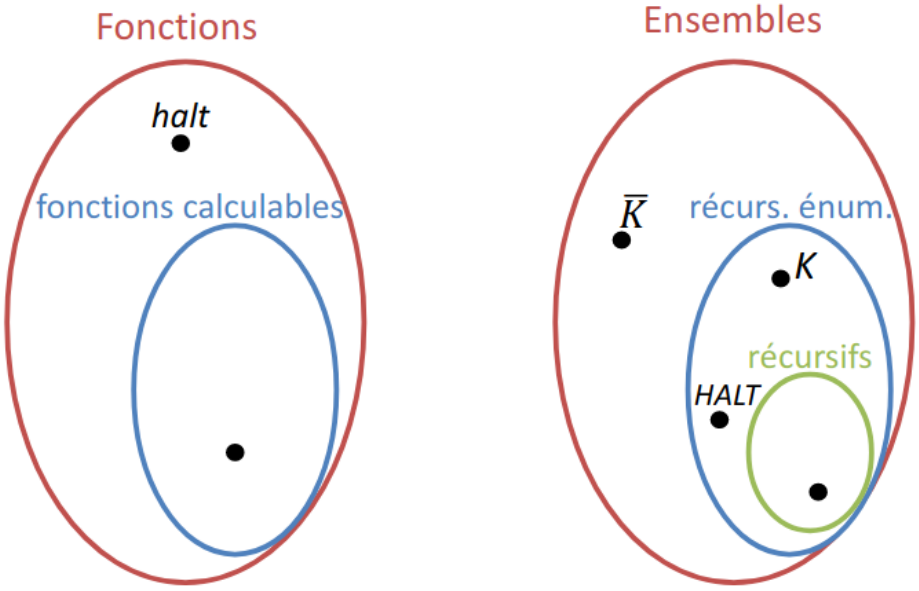
\includegraphics[width=0.4\textwidth,keepaspectratio]{fonctions_vs_ensembles}
\end{figure}

\subsection{Hoare-Allison}

Soit un langage $Q$ (non trivial) qui a des programmes $Q_k$ et qui ne calcule que des fonctions totales :
\begin{itemize}
\item La fonction $\varphi'_k$ est calculée par le programme $Q_k$
\item L'interpréteur $interpret(n,x)$ de ce langage $Q$ est calculable (p.ex. en Python)
\item La fonction $halt(n,x)$ pour ce langage $Q$ est calculable (fonction constante qui vaut 1)
\item \blue{$interpret(n, x)$ n'est pas calculable \textit{dans $Q$}}
\end{itemize}

\subsubsection{Preuve}

Supposons $interpret$ calculable dans $Q$.

\begin{enumerate}
\item \blue{Construire la table}
	\begin{figure}[H]
    		\centering
    		\begin{tabular}{c|cccccc}
		 & 0 & $\cdots$ & $k$ & $\cdots$ \\ 
		\hline 
		$Q_0$ & $interpret(0,0)$ & $\cdots$ & $interpret(0,k)$ & $\cdots$ \\
		$\vdots$ & $\vdots$ & $\ddots$ & $\vdots$ & $\cdots$ \\ 
		$Q_k$ & $interpret(k,0)$ & $\cdots$ & $interpret(k,k)$ & $\cdots$ \\ 
		$\vdots$ & $\vdots$ & $\vdots$ & $\vdots$ & $\ddots$ \\ 
		\end{tabular}
		\caption{Table des valeurs de la fonction $interpret$}
	\end{figure}
\item \blue{Prendre la diagonale} : $d(n) = interpret(n,n)$
\item \blue{Modifier la diagonale} : $d'(n)= interpret(n,n) + 1$ (calculable dans $Q$ si $interpret$ calculable dans $Q$)
\item \blue{Contradiction} : $d'(d)= interpret(d,d) + 1 \text{ \red{OR} } d'(d) = \varphi'(d) = interpret(d,d)$
\item \blue{Conclusion} : $interpret(n, x)$ n'est pas calculable dans $Q$
\end{enumerate}

\subsubsection{Interprétation}

Si un langage de programmation (non trivial) ne permet de calculer que des fonctions totales, alors :
\begin{itemize}
\item L'interpréteur de ce langage n'est pas calculable dans ce langage
\item Il existe des fonctions totales non programmables dans ce langage
\item Ce langage est dit restrictif
\end{itemize}

\subsubsection{Conséquences}

L'ensemble $\{n | \varphi_n \text{est totale} \}$ n'est pas récursif.
\begin{formal}
Tout formalisme utilisé pour étudier la calculabilité doit permettre de définir son propre interpréteur.
\begin{equation*}
\exists \ z \ \forall n, x : \varphi_z(n, x) = \varphi_n (x)
\end{equation*}
\begin{flushright}
Avec $\varphi_z$ la fonction calculée par l'interpréteur $P_z$
\end{flushright}
\end{formal}

\subsection{Rice}\label{dem:Rice}

Deux formulations :
\begin{enumerate}
\item Soit $A \subseteq \mathbb{N}$, si $A$ récursif, $A \neq \varnothing$ et $A \neq \mathbb{N}$ alors $\exists i \in A$ et $\exists j \in \bar{A}$ t.q. $\varphi_i = \varphi_j$
\item Si $\forall i \in A$ et $\forall j \in \bar{A} \ : \ \varphi_i \neq \varphi_j$ alors $A$ non récursif ou $A = \varnothing$ ou $A = \mathbb{N}$
\end{enumerate}
$\rightarrow$ Aucun programme ne peut dire si une fonction respecte des spécifications

\blue{Si A $\neq \varnothing$ et $A \neq \mathbb{N},\ \forall i \in A, \forall j \in \bar{A} \ : \ \varphi_i \neq \varphi_j$. Alors A non récursif.}

\subsubsection{Preuve}

\begin{enumerate}
\item On suppose $A$ récursif.\\
	On pose $P_k(x) \equiv$ while(True) $($c.à.d. $\varphi_k = \bot)$.\\
	Si $k \in \bar{A}$, comme $A \neq \varnothing \Rightarrow \exists m \in A$ et $\varphi_k \neq \varphi_m$
\item Construire $halt$ :
	\begin{equation*}
		 halt(n,x) \equiv
		 \begin{cases}
		 \text{Construire le programme (sans l'exécuter) } P(z) \equiv P_n(x); P_m(z)\\
		 d = \text{ numéro du programme }P(z)\\
		 \text{if } d \in A \text{ then } print(1) \ \green{\text{Si }P_n \text{ se termine, } \varphi_d = \varphi_m \rightarrow d \in A}\\
		 \text{else } print(0) \ \green{\text{Si }P_n \text{ ne se termine pas, } \varphi_d = \varphi_k \rightarrow d \in \bar{A}}\\
		 \end{cases}
	\end{equation*}
\item $halt$ n'est pas calculable, donc $A$ est non récursif
\end{enumerate}

\subsubsection{Signification et conséquences}

Si $A$ est récursif, qu'il n'est pas vide et qu'il ne contient pas l'ensemble des programmes existants, alors il existe un programme dans $A$ et un programme dans $\bar{A}$ tel qu'ils calculent la même fonction.

Sa conséquence la plus utile est sa contraposée : Si $\forall i \in A$ et $\forall j \in \bar{A}$, on a $\varphi_i \neq \varphi_j$, alors $A$ non-récursif ou $A = \emptyset$ ou $A = \mathbb{N}$.

Comme il est souvent simple de garantir $A = \emptyset$ et $A = \mathbb{N}$, on a un bon moyen de prouver que $A$ est non-récursif.

\subsubsection{Exemple d'application}

Soit $A = \{i \ |\ \varphi_i \text{ est totale}\}$
\begin{itemize}
\item $A \neq \emptyset$ : on peut écrire que $P_k \equiv$ print("Hello there")\\
	$k \in A \rightarrow A \neq \emptyset$
\item $A \neq \mathbb{N}$ : on peut écrire que $P_d \equiv$ while $True \ \{\}$ doSomething()
	$d \in A \rightarrow A \neq \mathbb{N}$
\item $\forall i \in A, \forall j \in \bar{A}\ :\ \varphi_i$ est total tandis que $\varphi_j$ ne l'est pas $\rightarrow$ pas égaux
\end{itemize}
Donc, $A$ n'est pas récursif.

\subsection{Paramétrisation}

Si un programme $P(a,b)$ existe, alors il existe un programme $P'_b(a)$ (où b est fixé) t.q. $P'_b(a) \equiv Exec \ P(a,b)$

\subsubsection{Forme S-1-1}

Il existe une fonction totale calculable $S^1_1 : \mathbb{N}^2 \rightarrow \mathbb{N}$ t.q. $\forall k : \varphi_k(x_1, x_2) = \varphi_{S^1_1(k,x_2)}(x_1)$

\subsubsection{Forme S-m-n}

$\forall m,n \geq 0, \exists$ une fonction totale calculable $S^m_n : \mathbb{N}^{m+1} \rightarrow \mathbb{N}$ t.q. $\forall k : \varphi_k(x_1, \ldots, x_n, x_{n+1}, \ldots, x_{n+m}) = \varphi_{S^1_1(k,x_{n+1}, \ldots, x_{n+m})}(x_1, \ldots, x_n)$

\newpage
\subsection{Point fixe}

Soit $f$ une fonction totale calculable. Il existe $k$ t.q. $\varphi_k = \varphi_f(k)$.

\subsubsection{Preuve}

On pose :
\begin{equation}\label{eq:pf1}
h(u,x) =
\begin{cases}
	\varphi_{\varphi_u(u)}(c) & \text{si}\ \varphi_u(u) \neq \bot\\
	\bot & \text{sinon}
\end{cases}
\end{equation}
\begin{itemize}
\item[] Où $h(u,x)$ est calculable
\end{itemize}
\begin{equation}\label{eq:pf2}
h(u,x) = \varphi_{S(u)}(x)
\end{equation}
\begin{itemize}
\item[] Par application de $S-1-1$
\end{itemize}
\begin{equation}\label{eq:pf3}
g(x) = f(S(x))
\end{equation}
\begin{itemize}
\item[] Où $g$ est totale calculable (car $f$ et $S$ le sont),
\item[] et $f$ est donné par $k' : \varphi_{k'}(x) = g(x) = f(S(x))$.
\end{itemize}

\medskip

On a que $k'$ est une constante par l'équation \ref{eq:pf2} :
\begin{equation*}
h(k',x) = \varphi_{S(k')}(x)
\end{equation*}

Par l'équation \ref{eq:pf1} et comme $g = \varphi_{k'}$ :
\begin{equation*}
h(k',x) = \varphi_{k'(k')}(x)
\end{equation*}

Par l'équation \ref{eq:pf3}, on a que $\varphi_{k'} = g(x) = f(S(x))$, donc :
\begin{equation*}
h(k',x) = \varphi_{f(S(x))}(x)
\end{equation*}

Si on pose que $S(k') = k$, on obtient :
\begin{equation*}
\varphi_k(x) = \varphi_{f(k)}(x)
\end{equation*}

\subsubsection{Analyse}

Pour tout transformateur de programme $T$, il existe deux programmes $P_k$ et $P_j$ t.q. :
\begin{itemize}
\item $P_j$ est la transformation de $P_k$ via $T$
\item $P_j$ et $P_k$ calculent la même chose.
\end{itemize}

\subsubsection{Exemple}

$K = \{n\ |\ \varphi_n(n) \neq \bot \}$. Soient $f_n(x) = \bot\ \forall x$ et $f_m(x) = x\ \forall x$

Définition de $f(x) =
\begin{cases}
	n & \text{si}\ x \in K\\
	m & \text{sinon}
\end{cases}$ $f$ est totale calculable si $K$ récursif.

Point fixe : $\exists k : \varphi_k = \varphi_{f(k)}$
\begin{itemize}
\item Si $k \in K$
	\begin{itemize}
	\item Par définition de $f$ : $f(k) = n$
	\item Par point fixe : $\varphi_k (k) = \varphi_n(k) \rightarrow$ \red{Contradiction}
	\end{itemize}
\item Si $k \notin K$
	\begin{itemize}
	\item Par définition de $f$ : $f(k) = m$
	\item Par point fixe : $\varphi_k(k) = \varphi_m(k) \rightarrow$ \red{Contradiction}
	\end{itemize}
\end{itemize}

\chapter{Modèles}

\section{Familles de modèles}

\begin{enumerate}
\item Modèles basées sur le calcul :
	\begin{itemize}
	\item Déterministes (une exécution)
	\item Non-Déterministes (plusieurs exécutions possibles)
	\end{itemize}
\item Modèles basés sur le langage
\end{enumerate}

\section{Langages de programmation}

\subsection{Définition}

\begin{itemize}
\item Syntaxe
\item Sémantique
\item Convention de représentation d'une fonction par un programme
\end{itemize}

\subsection{Langages complets}

Langages tel que : Oz, Python, JS, C, etc. sont (en terme de calculabilité) équivalent. Ils permettent de calculer les mêmes fonctions.

\subsection{BLOOP (Bounded Loop)}

Un programme BLOOP est un programme Python tel que :
\begin{itemize}
\item Pas de boucle while
\item Boucle for limité (pour que la boucle se termine quoi qu'il arrive)
\item Pas de méthode récursive
\end{itemize}

\subsubsection{Propriétés}

\begin{itemize}
\item Tous les programmes BLOOP se terminent
\item BLOOP ne calcule que des fonctions totales (mais ne les calcule pas toutes les Hoare-Allison)
\item Il existe un compilateur des programmes BLOOP
\item BLOOP n'est pas un modèle complet de la calculabilité
\end{itemize}

\subsection{ND-Java}

C’est un sous-ensemble de Java (“Non-Deterministic Java”)
On y ajoute fonction $choose(n)$ renvoyant un entier aléatoire entre 0 et $n$. Cette \blue{fonction est non-déterministe} car à un même input elle ne renvoie pas toujours le même output.

\subsection{ND-Récursif}

$A$ est ND-Récursif si $\exists$ un programme ND-Java t.q. s'il reçoit un input $x \in \mathbb{N}$ :
\begin{itemize}
\item $x \in A$ alors $\exists$ une exécution qui retourne 1
\item $x \notin A$ alors pour toute exécution le résultat est 0
\end{itemize}

\subsubsection{ND-Récursif énumérable}

Comme ND-Récursif sauf que le cas $x \notin A$ ne se fini pas forcément.

\subsubsection{Propriétés}

\begin{itemize}
\item Récursif $\Rightarrow$ ND-Récursif
\item Récursif énumérable $\Rightarrow$ ND-Récursif énumérable
\end{itemize}

\section{Automates Finis (FA)}

Objectif : décider si un mot appartient ou non à un langage.
\begin{itemize}
\item Nombre fini d'états
\item Lecture d'une donnée (mot : string)
\item Chaque symbole lu \textit{une fois}
\item Transitions entre états en fonction du symbole
\item État final = après avoir tout lu
\item Pas de mémoire
\end{itemize}

\subsection{Composition}

\begin{itemize}
\item $\Sigma$ : ensemble (fini) de symboles
\item $S$ : ensemble (fini) d'états
\item $S_0 \in S$ : état initial
\item $A \subseteq S$ : ensemble des états acceptants
\item $\delta : Sx\Sigma \rightarrow S$ : fonction de transition
\end{itemize}

\subsection{Exemple}

\begin{figure}[H]
    \centering
    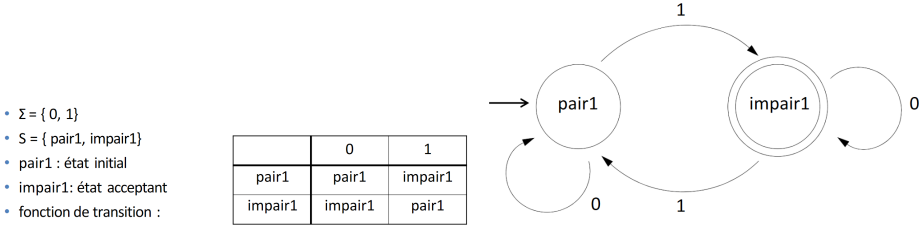
\includegraphics[width=\textwidth,keepaspectratio]{fa}
    \caption{Exemple d'un automate fini (déterministe)}
\end{figure}

Un automate détermine un ensemble récursif $\{m\ |\ m$ accepté par le FA$\}$. En contrepartie, il ne peut pas programmer son interpréteur.

\subsection{ND-FA}

Non déterministe $\rightarrow \{m\ |$ s'il existe une exécution où $m$ est accepté par le FA$\}$

\begin{figure}[H]
    \centering
    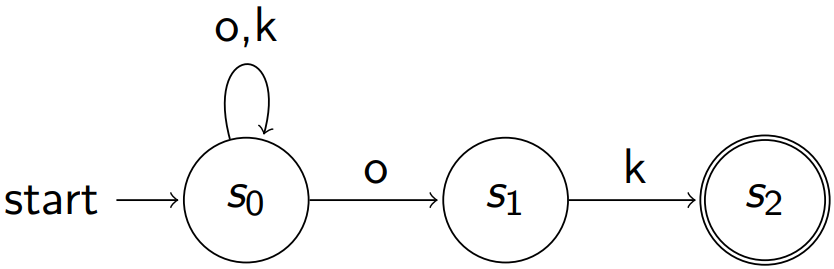
\includegraphics[width=0.6\textwidth,keepaspectratio]{ndfa}
    \caption{Exemple d'un automate fini non-déterministe}
\end{figure}

\subsubsection{$\epsilon$-NDFA}

Il peut y avoir des transitions vides.

\newpage
\section{Machines de Turing}

\begin{figure}[H]
    \centering
    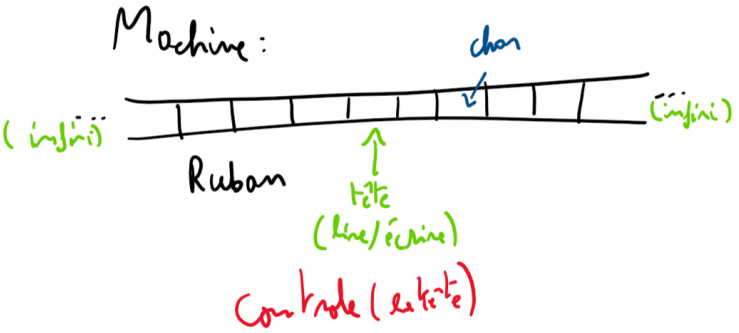
\includegraphics[width=0.6\textwidth,keepaspectratio]{turing}
\end{figure}

\begin{itemize}
\item \textbf{Ruban} : infini des deux côtés (mais à un moment $n$ de l'exécution, il y a un nombre fini de cases allouées)
\item \green{Tête} : sur une seule case à la fois. Elle peut lire et écrire
\item \red{Contrôle} : dirige la tête sur le ruban
\end{itemize}

\subsection{États}

\begin{itemize}
\item Début
\item Arrêt (le ruban = le résultat)
\item Autres (pendant l'exécution)
\end{itemize}

\subsection{Déplacement}

\begin{equation*}
<q, c>\ \rightarrow\ <new\_q, Mouv, new\_c>
\end{equation*}
Avec :

\begin{itemize}
\item \blue{$q$} : l'état courant ($\neq$ état marchant)
\item \blue{$c$} : symbole sous la tête de lecture
\item \blue{$new\_c$} : symbole à écrire sous la tête de lecture (avant le mouvement)
\item \blue{$Mouv$} : mouvement (Droite ou Gauche) à faire (1 case à la fois)
\item \blue{$new\_q$} : état suivant
\end{itemize}

\subsection{Modélisation}

\begin{itemize}
\item $\Sigma$ : ensemble fini de symboles d'entrée
\item $\Gamma$ : ensemble fini de symboles du ruban (ce qui peut être écrit sur le ruban)
	\begin{itemize}
	\item $\Sigma \subset \Gamma$ (les symboles d'entrée peuvent être écrit sur le ruban)
	\item $B \in \Gamma, B \notin \Sigma$ (symbole blanc = par défaut sur les cases vides)
	\end{itemize}
\item $S$ : ensemble fini d'états
\item $S_0 \in S$ : état initial
\item \textit{stop} $\in S$ : état d'arrêt
\item $\delta : S\text{x}\Gamma\ \rightarrow\ S\text{x}\{G,D\}\text{x}\Gamma$ : fonction de transition (fini)
\end{itemize}

\newpage
\subsection{Exécution}

\begin{figure}[H]
    \centering
    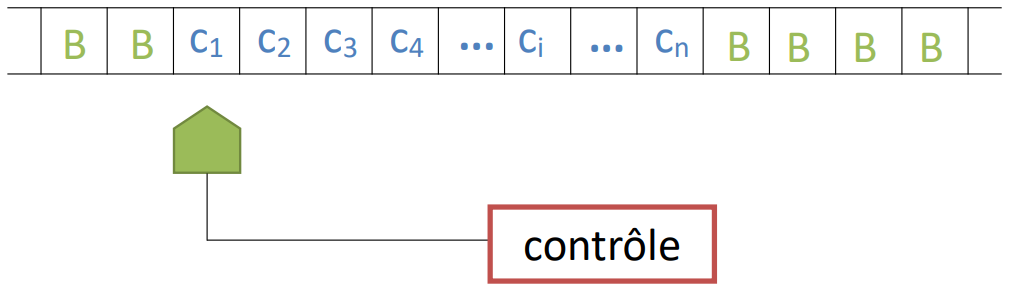
\includegraphics[width=0.35\textwidth,keepaspectratio]{turing_exec_1}
\end{figure}
\begin{itemize}
\item Données sur le ruban ($c_1, c_2, c_3, ..., c_n$)
\item Autres cases contiennent le symbole blanc ($B$)
\item Tête de lecture initialement sur la première case de la donnée
\item Tant que des instructions sont applicables, le contrôle applique les instructions
\item L'exécution s'arrête dès que l'état devient \textit{stop}
\item S'il n'y a pas d'instruction applicable, il y a un arrêt
\item Résultat : contenu du ruban à l'état \textit{stop} ($d_1, d_2, d_3, ..., d_m$)
\end{itemize}
\begin{figure}[H]
    \centering
    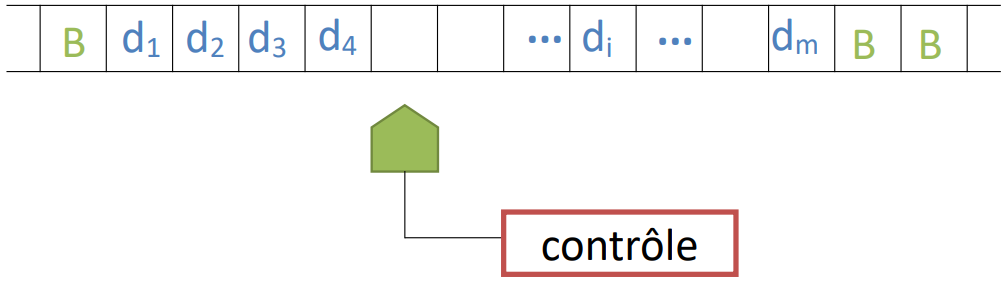
\includegraphics[width=0.35\textwidth,keepaspectratio]{turing_exec_2}
\end{figure}

\subsection{Exemple}

Machine de Turing calculant la fonction $f(x) = x+1$.
\begin{itemize}
\item Représentation des entier sous forme binaire
\item $\Sigma = \{0, 1\}$
\item $\Gamma = \{0, 1, B\}$
\end{itemize}
\begin{figure}[H]
    \centering
    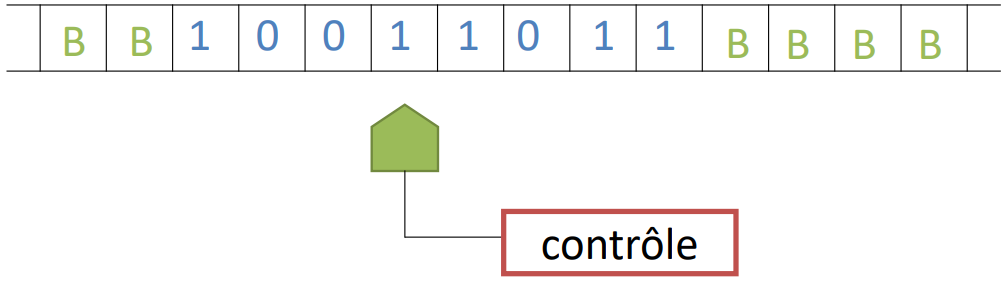
\includegraphics[width=0.35\textwidth,keepaspectratio]{turing_ex_1}
\end{figure}
\begin{enumerate}
\item Positionner la tête de lecture sur le bit de poids le plus faible
\item Réaliser l'addition et les reports nécessaires
\item Report final et fin
\end{enumerate}

\begin{minipage}{0.49\textwidth}
	\begin{figure}[H]
		\centering
		\legend{\blue{Exécution}}
		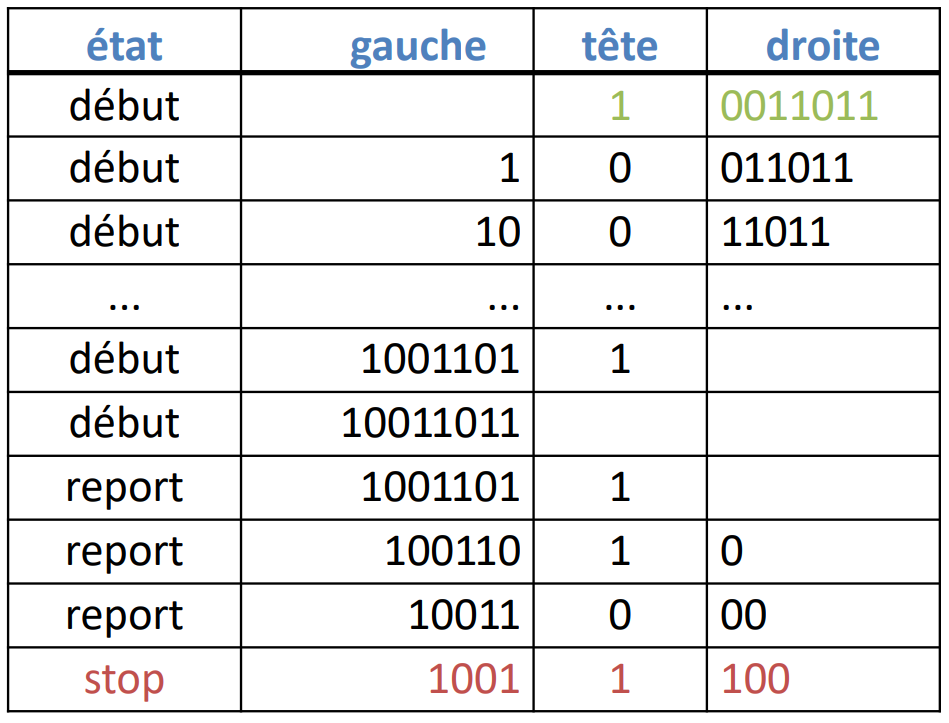
\includegraphics[width=0.8\textwidth,keepaspectratio]{turing_ex_2}
	\end{figure}
\end{minipage}
\begin{minipage}{0.49\textwidth}
	\begin{figure}[H]
		\centering
		\legend{\blue{Positionner la tête de lecture à droite}}
		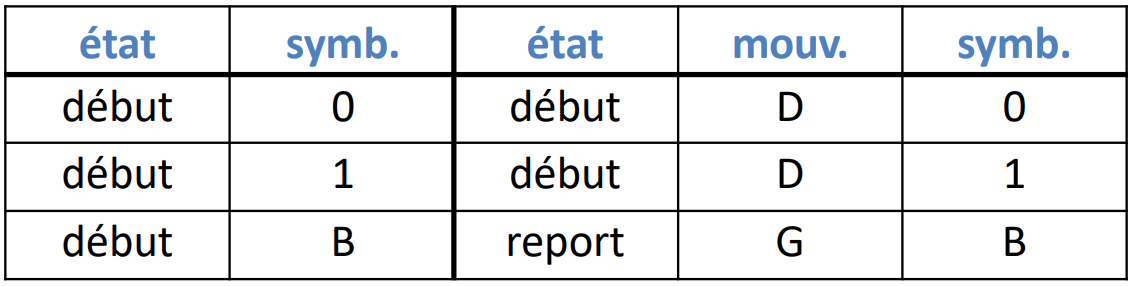
\includegraphics[width=0.8\textwidth,keepaspectratio]{turing_ex_2_1}
	\end{figure}
	\begin{figure}[H]
		\centering
		\legend{\blue{Addition}}
		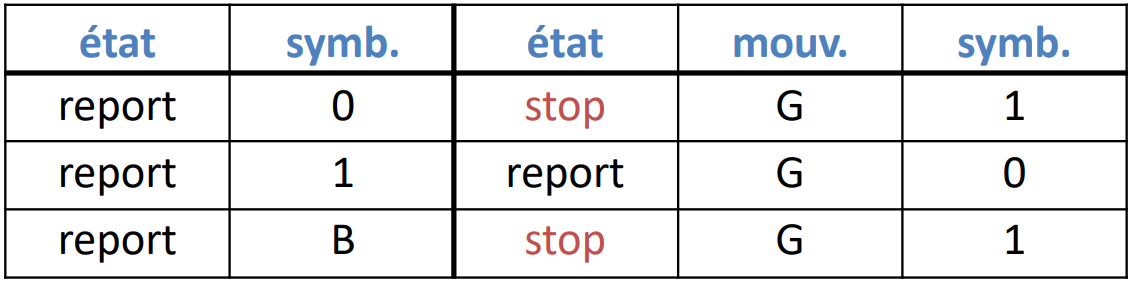
\includegraphics[width=0.8\textwidth,keepaspectratio]{turing_ex_2_2}
	\end{figure}
\end{minipage}

\chapter{Classes de complexité}

\section{Réduction et ensemble complet}

But : on a un problème $P$,et on va le \textit{déduire} à partir d'un problème $P'$.

\section{Réduction algorithmique (calculabilité)}

Un ensemble $A$ est \blue{algorithmiquement réductible} à un ensemble $B \ (A \leq_a B)$ si en supposant $B$ récursif, $A$ est récursif.

Exemple :

Soit $P = \{n \ | \ \varphi_n$ renvoi un nombre pair $\}$ : $HALT \ \leq_a P$ (si $P$ énumérable, $HALT$ énumérable)

\subsection{Ensemble complet}

Étant donné une classe $A$ de problèmes dont $E$ est le problème le plus difficile :
\begin{figure}[H]
    \centering
    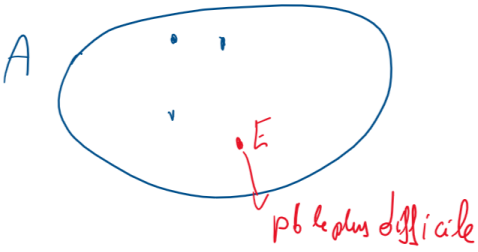
\includegraphics[width=0.35\textwidth,keepaspectratio]{ensemble_complet}
\end{figure}
On dit que le problème $E$ est $A$-complet par rapport à une relation de réduction ($\leq_a$) ssi :
\begin{enumerate}
\item $E \in A$
\item $\forall B \in A : B \leq_a E$
\end{enumerate}
On dit que le problème $E$ est $A$-difficile par rapport à une relation de réduction ($\leq_a$) ssi :
\begin{enumerate}
\item $\forall B \in A : B \leq_a E$
\end{enumerate}

\subsection{Propriétés}

\begin{itemize}
\item Si $A \leq_a B$ et $B$ récursif, alors $A$ récursif
\item Si $A \leq_a B$ et $B$ récursivement énumérable, alors $A$ pas nécessairement énumérable
\item Si $A \leq_a B$ et $A$ non récursif, alors $B$ non récursif
\item $A \leq_a \bar{A}$
\item $A \leq_a B \Leftrightarrow \bar{A} \leq_a B$
\item Si $A$ récursif, alors pour tout $B$, $A \leq_a B$
\end{itemize}

\section{Réduction fonctionnelle (complexité)}

Un ensemble $A$ est \blue{fonctionnellement réductible} à un ensemble $B \ (A \leq_f B)$ ssi il existe une fonction totale calculable $f$ t.q. :
\begin{equation*}
a \in A \Leftrightarrow f(a) \in B
\end{equation*}

Pour décider si un élément appartient à $A$, il suffit de :
\begin{enumerate}
\item Calculer $f(a)$
\item Tester si $f(a) \in B$
\end{enumerate}

\subsection{Propriétés}

\begin{itemize}
\item Si $A \leq_f B$ et $B$ récursif, alors $A$ récursif
\item Si $A \leq_f B$ et $B$ récursif énumérable, alors $A$ récursif énumérable
\item Si $A \leq_f B$ et $A$ non récursif, alors $B$ non récursif
\item $A \leq_f B \leftrightarrow \bar{A} \leq_f \bar{B}$
\item Si $A$ récursif, alors pour tout $B$, $A \leq_f B$
\item Pas nécessairement $A \leq_f \bar{A}$
\item Si $A \leq_f B$, alors $A \leq_b B$ (l'inverse n'est pas nécessairement vrai)
\end{itemize}

\section{Modèle de calcul}

Tout les modèles de complexité ont entre eux des complexité spatiales et temporelles reliées de façon polynomiale.

\subsection{Conséquence}

Si un programme est faisable dans un modèle (non déterministe), alors il est pratiquement faisable dans tous les modèles (non déterministes). Concrètement, entre une MT et un programme Python, il y aura des différences de complexité mais elles resteront polynomiales.

\section{Classes de complexité}

\begin{itemize}
\item $DTIME(f)$ : Ensemble récursif décidé par un programme Python en complexité temporelle $\bigO(f)$
\item $DSPACE(f)$ : Ensemble récursif décidé par un programme Python en complexité spatiale $\bigO(f)$
\item $NTIME(f)$ : Ensemble ND-récursif décidé par un programme Python en complexité temporelle $\bigO(f)$ (sur toutes les branches)
\item $NSPACE(f)$ : Ensemble ND-récursif décidé par un programme Python en complexité spatiale $\bigO(f)$ (sur toutes les branches)
\item Classe $P$ (Polynomiale): $P = \underset{i \geq 0}{\bigcup} DTIME(n^i)$
\item Classe $NP$ (Non-Polynomiale): $P = \underset{i \geq 0}{\bigcup} NTIME(n^i)$
\end{itemize}

\section{Relations entre classes de complexité}

\subsection{Déterministe VS non déterministe}

\begin{itemize}
\item Si $A \in NTIME(f)$ alors $A \in DTIME(c^f)$
\item Si $A \in NSPACE(f)$ alors $A \in DSPACE(f^2)$
\end{itemize}

\subsection{Time VS Space}

\begin{itemize}
\item Si $A \in NTIME(f)$ alors $A \in NSPACE(f)$
\item Si $A \in DTIME(f)$ alors $A \in DSPACE(f)$
\item Si $A \in NSPACE(f)$ alors $A \in NTIME(c^f)$
\item Si $A \in DSPACE(f)$ alors $A \in DTIME(c^f)$
\end{itemize}

\section{NP-complétude}

\begin{equation*}
\text{Si } A \in P\ \rightarrow\ A \in NP\ ? \rightarrow \text{ On ne sait pas}
\end{equation*}

\subsection{Réduction polynomiale}

Un ensemble $A$ est \blue{polynomialement réductible} à un ensemble $B \ (A \leq_p B)$ ssi il existe une fonction totale calculable $f$ de complexité temporelle polynomiale t.q. :
\begin{equation*}
a \in A \Leftrightarrow f(a) \in B
\end{equation*}

Si $A \leq_p B$ et $B \in P$ alors $A \in P$.

\subsection{NP-complétude}

Un problème $E$ est $NP$\footnote{NP = Non-déterministe Polynomiale}-complet ($\leq_p$) ssi :
\begin{enumerate}
\item $E \in NP$
\item $\forall B \in NP : B \leq_p E$
\end{enumerate}
Un problème $E$ est $NP$-difficile ($\leq_p$) ssi :
\begin{enumerate}
\item $\forall B \in NP : B \leq_p E$
\end{enumerate}

\subsubsection{Propriétés}

Soit $E$ un ensemble $NP$-complet
\begin{itemize}
\item $E \in P$ ssi $P = NP$
\item $E \notin P$ ssi $P \neq NP$
\item Si $E \leq_p B$ et $B \in NP$, alors $B$ est $NP$-complet
\end{itemize}

\chapter{Analyse et Perspectives}

\section{Fondement de la thèse de Church-Turing}

Forme originale :
\begin{itemize}
\item \blue{Première partie} : Toute fonction calculable par une machine de Turing est effectivement calculable
\item \blue{Deuxième partie} : Tout fonction effectivement calculable est calculable par une machine de Turing
\end{itemize}

Ici, en parlant de Machine de Turing, on parle d'un modèle de calculabilité (pourrait être Python par exemple).

\section{Formalismes de calculabilité}

Soit $D$ un nouveau formalisme de calculabilité :

\subsection{Caractéristiques de formalisme}

\begin{itemize}
\item $SD$ (Soudness des Descriptions) : toute fonction $D$-calculable est calculable
\item $CD$ (Complétude des Définitions) : toute fonction calculable est $D$-calculable
\item $SA$ (Soudness Algorithmique) : l'interpréteur de $D$ est calculable
\item $CA$ (Complétude Algorithmique) : si $p \in P$ ($P$ est par exemple Java), que $p' \in D$ et que $p \equiv p'$ (calculent la même fonction), alors équivalence des formalismes
\item $U$ (Description Universelle) : l'interpréteur de $D$ est $D$-calculable
\item $S$ ($S-m-n$ Affaiblie) : $\forall d \in D \ \exists S : d(x,y) = [S(x)](y)$
\end{itemize}

\subsection{Propriétés}

\begin{itemize}
\item $SA \Rightarrow SD$
\item $CA \Rightarrow CD$
\item $SD$ et $U \Rightarrow SA$
\item $CD$ et $S \Rightarrow CA$
\item $SA$ et $CD \Rightarrow U$
\item $CA$ et $SD \Rightarrow S$
\item $S$ et $U \Rightarrow S-m-n$
\item $SA$ et $CA \Leftrightarrow SD$ et $CD$ et $U$ et $S$
\item $SA$ et $CD$ et $S \Leftrightarrow CA$ et $SD$ et $U$
\end{itemize}

Exemple : BLOOP est $SD$, $SA$, et $S$ mais pas le reste.

\chapter{Preuves supplémentaires}

\section{L'ensemble des fonctions totales n'est pas énumérable}\label{sec:ensembleF}

Soit $F$ l'ensemble des fonctions totales telles que $f : \mathbb{N} \rightarrow \mathbb{N}$.

\blue{$F$ est non énumérable}.

\subsubsection*{Preuve}

Supposons $F$ énumérable. Il existe donc une énumération des éléments de $F : f_0(0), f_1(0), \ldots$.

\begin{enumerate}
\item \red{Construire la table}
	\begin{figure}[H]
    		\centering
    		\begin{tabular}{c|cccccc}
		 & 1 & 1 & 2 & $\cdots$ & $k$ & $\cdots$ \\ 
		\hline 
		$f_0$ & $f_0(0)$ & $f_0(1)$ & $f_0(2)$ & $\cdots$ & $f_0(k)$ & $\cdots$ \\ 
		$f_1$ & $f_1(0)$ & $f_1(1)$ & $f_1(2)$ & $\cdots$ & $f_1(k)$ & $\cdots$ \\ 
		$f_2$ & $f_2(0)$ & $f_2(1)$ & $f_2(2)$ & $\cdots$ & $f_2(k)$ & $\cdots$ \\ 
		$\vdots$ & $\vdots$ & $\vdots$ & $\vdots$ & $\ddots$ & $\vdots$ & $\cdots$ \\ 
		$f_k$ & $f_k(0)$ & $f_k(1)$ & $f_k(2)$ & $\cdots$ & $f_k(k)$ & $\cdots$ \\ 
		$\vdots$ & $\vdots$ & $\vdots$ & $\vdots$ & $\vdots$ & $\vdots$ & $\ddots$ \\ 
		\end{tabular}
		\caption{Table des résultats de la fonction $f$}
	\end{figure}
\item \red{Prendre la diagonale} $d$ qui est aussi une fonction de $\mathbb{N} \rightarrow \mathbb{N} \ (d \in F)$
\item \red{Modifier la diagonale} pour obtenir $d'$ t.q. :
	\begin{equation*}
		f'_i(j)=
		\begin{cases}
      		5 & \text{si}\ f_i(j) \neq 5\\
      		6 & \text{sinon}\
      	\end{cases}
    \end{equation*}
    
    Où $f_i(j)$ est le résultat de la fonction $f$ avec le numéro $i$ pour la donnée $j$.
\item \red{Contradiction} :

	Comme $F$ est énumérable et que $d' \in F$, alors $d'$ doit être dans l'énumération. Or si $d'$ a le numéro $p$ on a :
	\begin{align*}
		d' &= f_p(0),f_p(1),f_p(2),\ldots,f_p(p),\ldots\\
		   &= f'_p(0),f'_p(1),f'_p(2),\ldots,f'_p(p),\ldots\\
    \end{align*}
    Si $f_p(0)$ vaut 5, on a $(f_p(0) = 5) \neq (f'_p(0) = 6)$.
\item \red{Conclusion} :

	$F$ n'est pas énumérable.
\end{enumerate}

\section[P = NP]{Si $SAT \in P$ alors $P = NP$}\label{dem:PNP}

Le théorème de Cook dit que $SAT$ est NP-complet. Cela implique :
\begin{enumerate}
\item $SAT \in NP$
\item $\forall B \in NP : B \leq_p SAT$
\end{enumerate}

Un ensemble $A$ est polynomialement réductible à un ensemble $B$, $A \leq_p B$ s'il existe une fonction totale calculable $f$ de complexité temporelle polynomiale telle que :

\begin{equation*}
a \in A \Leftrightarrow f(a) \in B
\end{equation*}

Comme $A \leq_p SAT$, $\forall A \in NP$, on pourrait alors réduire n'importe quel problème $NP$ à $SAT$ en complexité polynomiale puis résoudre $SAT$ en temps polynomiale également, ce qui entraînerait $P = NP$.
